%
% Apunte de Sistemas Operativos
% Copyright (C) 2014 Esteban De La Fuente Rubio (esteban[at]delaf.cl)
%
% Permission is granted to copy, distribute and/or modify this document
% under the terms of the GNU Free Documentation License, Version 1.3
% or any later version published by the Free Software Foundation;
% with no Invariant Sections, no Front-Cover Texts, and no Back-Cover Texts.
% A copy of the license is included in the section entitled "GNU
% Free Documentation License".
%
% Link: http://www.gnu.org/copyleft/fdl.html
%

% CAPÍTULO ESTRUCTURA Y DISEÑO
\chapter{Estructura y diseño}
\label{estructura}
El sistema operativo es el encargado de ofrecer diferentes servicios, tanto al
usuario como a otros procesos. Es importante mencionar que aquí se contrapondrán
los objetivos que tiene el sistema con los requerimientos de los usuarios.

A continuación se listan una serie de servicios que deben ser considerados al
momento de diseñar un sistema operativo, algunos de los cuales se discutirán en
mayor detalle más adelante.

\begin{enumerate}[a.]

	\item \textbf{Interfaz de usuario}: servicio que entrega un método para
	que el usuario pueda interactuar con el sistema operativo, ya sea una
	CLI o una GUI.

	\item \textbf{Ejecución de programas}: el sistema operativo se debe
	encargar de mantener a los procesos en ejecución durante todo su ciclo
	de vida, esto implica la administración de los mismos durante sus
	posibles estados de ejecución.

	\item \textbf{Operaciones de entrada/salida (E/S)}: un proceso no podrá
	acceder directamente a los recursos disponibles en la máquina, debe ser
	el sistema operativo quien, mediante una interfaz de acceso, permita a
	los diferentes procesos acceder a los dispositivos de entrada y salida
	de forma concurrente y controlada.

	\item \textbf{Sistema de archivos}: se debe proveer de una forma de
	acceder al disco con alguna estructura, donde no se deban escribir
	directamente posiciones de memoria, sino que los procesos puedan
	escribir y leer archivos dentro de los dispositivos.

	\item \textbf{Comunicación entre procesos (IPC o \textit{Inter Process
	Communication})}: corresponde al mecanismo que permite que diferentes
	procesos se comuniquen entre sí, por ejemplo mediante el uso de memoria
	compartida, \textit{sockets} o tuberías.

	\item \textbf{Detección de errores}: sistema deberá capturar los
	errores, tanto físicos como lógicos que un proceso pueda generar y
	evitar que dicho error afecte a otros procesos en ejecución.

	\item \textbf{Asignación de recursos}: los diferentes dispositivos en la
	máquina podrán ser utilizados concurrentemente por muchos procesos, por
	lo que deberá existir algún algoritmo que permita planificar quien
	utilizará un recurso en un momento dado.

	\item \textbf{Estadísticas}: estas son llevadas con propósitos
	contables, para detectar errores o para, por ejemplo, predecir el
	comportamiento futuro de un proceso y poder tomar decisiones de
	planificación al respecto.

	\item \textbf{Protección y seguridad}: el acceso a los recursos
	disponibles debe ser controlado, se debe evitar que cualquier proceso
	pueda utilizar cualquier dispositivo, en cualquier momento.

\end{enumerate}

\section{Interfaz de usuario}
Las \textbf{interfaces de usuario} permiten al usuario realizar una interacción
con el sistema operativo, se dividen básicamente en dos tipos
\textbf{\textit{Command Line Interface}} (CLI) y \textbf{\textit{Graphical User
Interface}} (GUI).

\subsection{CLI}
La interfaz de línea de comando, o simplemente la \textit{shell}, corresponde a
un intérprete en modo texto que permite introducir órdenes para que sean
ejecutadas por el sistema operativo. Su tarea principal es recibir las
solicitudes del usuarios, y en la mamyoría de los casos ejecutar un programa
asociado a dicha solicitud.

Algunos ejemplos de \textit{shells} conocidas en diferentes sistemas operativos
\textit{like Unix} son:

\begin{itemize}

	\item sh: Steve Bourne, Unix v7, 1978.

	\item ash: usada como base para las shell de BSD.

	\item bash: parte del proyecto GNU.

	\item dash: ash mejorada para Debian GNU/Linux.

\end{itemize}

La \textit{shell} ejecutará los comandos que el usuario introduzca, algunos de
ellos serán comándos básicos (como listar directorios, crear una carpeta, ver la
fecha) o podrían ser programas más complejos (como un editor de texto o una
aplicación en modo texto). Adicionalmente se puede utilizar un lenguaje de
programación para realizar \textit{scripts}, donde existe un estándar denominado
\textit{shell scripting}, sin embargo cada intérprete puede implementar
extensiones para el mismo.

Un comando al ser ejecutado deberá ser buscado dentro del PATH del sistema, el
cual corresponde a la ruta de directorios donde posiblemente se podría encontrar
dicho comando, si luego de revisar todos los directorios del PATH el comando no
es encontrado se informa al usuario. En caso de ser encontrado el comando puede
estar implementado como un programa externo de la \textit{shell} o como un
programa dentro de la \textit{shell}, como el caso de algunas extensiones. La
ventaja de utilizar el primer método, fuera del intérprete, es que no se debe
modificar este para agregar nuevos comandos, bastará agregarlos a alguna de las
rutas en el PATH.

En general la shell de un usuario no privilegiado (usuario normal) tendrá el
signo \$ y un usuario privilegiado (o sea, el usuario root) tendrá el signo \#
para indicar que está en espera del ingreso de comandos. De esta forma si vemos
un comando precedido por un signo \$, dicho comando se ejecuta como usuario sin
privilegios, en cambio si vemos un comando precedido por un signo \#
necesariamente dicho comando se debe ejecutar con el usuario root.

\subsection{GUI}
La interfaz de usuario gráfica corresponde al entorno de ventanas, el cual
permite tener diversas aplicaciones encapsuladas dentro de un cuadro (ventana) y
de esta forma compartir de manera fácil un único recurso, la pantalla, con
múltiples procesos que quieren dibujar en ella. En sistemas \textit{like Unix}
es conocido como X en honor a Xerox que lo ideo en los años 70s\footnote{¡Si!
mucho antes que Microsoft Windows empezara a usarlas}.

Algunos entornos de escritorio y gestores de ventanas son KDE, Gnome, XFCE,
Lxde, Fluxbox y OpenBox. Algunos de estos pueden apreciarse en la figura
\ref{gui}.

El entorno gráfico no es propiamente una función del sistema operativo, de hecho
es una aplicación más que funciona sobre este, la cual entrega una forma ``más
amigable'' de interactuar con el sistema.

\begin{figure}[htbp]
\begin{center}
	\subfigure[KDE 3.5]{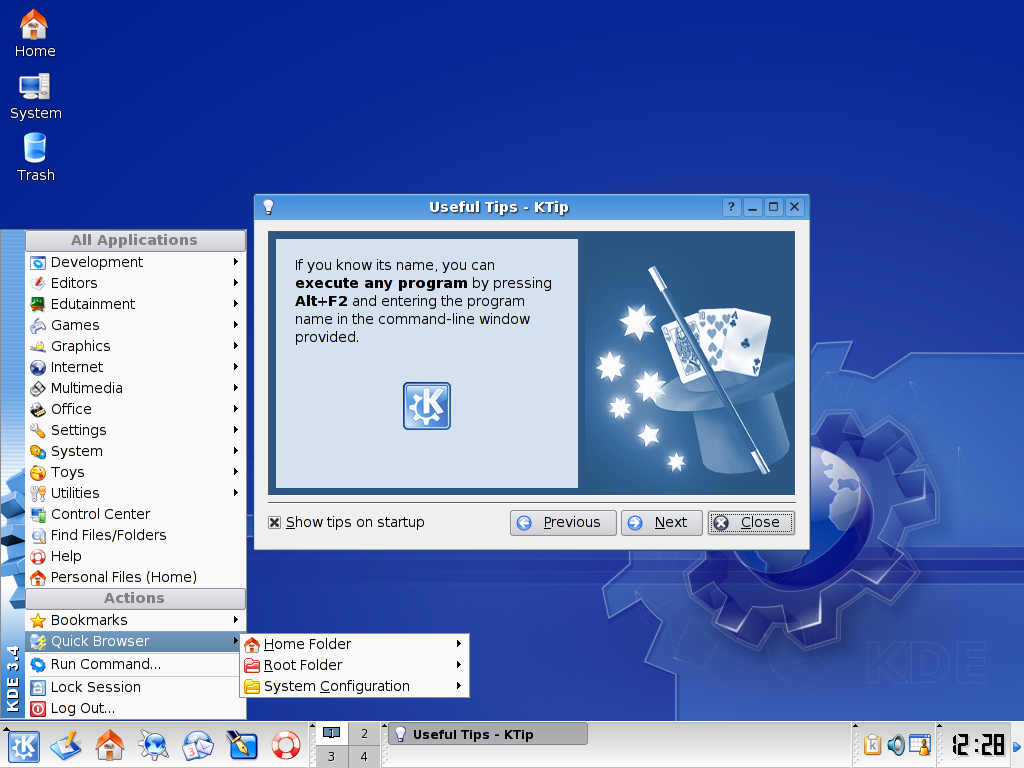
\includegraphics[height=3.5cm]{img/C03_estructura/gui_kde35}}
	\subfigure[KDE 4]{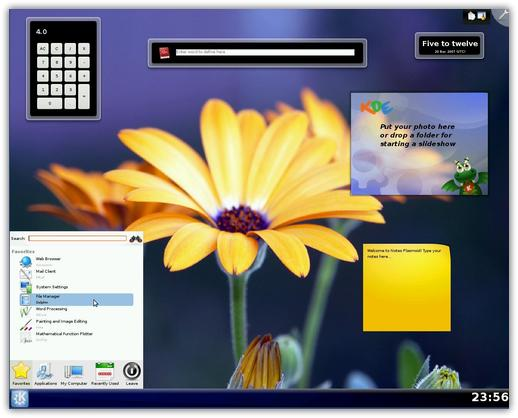
\includegraphics[height=3.5cm]{img/C03_estructura/gui_kde4}}
	\subfigure[Gnome]{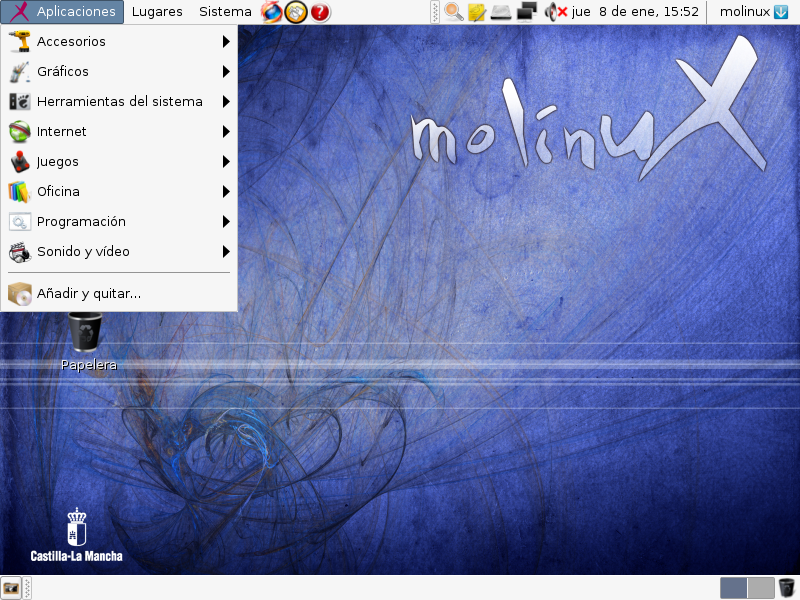
\includegraphics[height=3.5cm]{img/C03_estructura/gui_gnome}}
	\subfigure[XFCE]{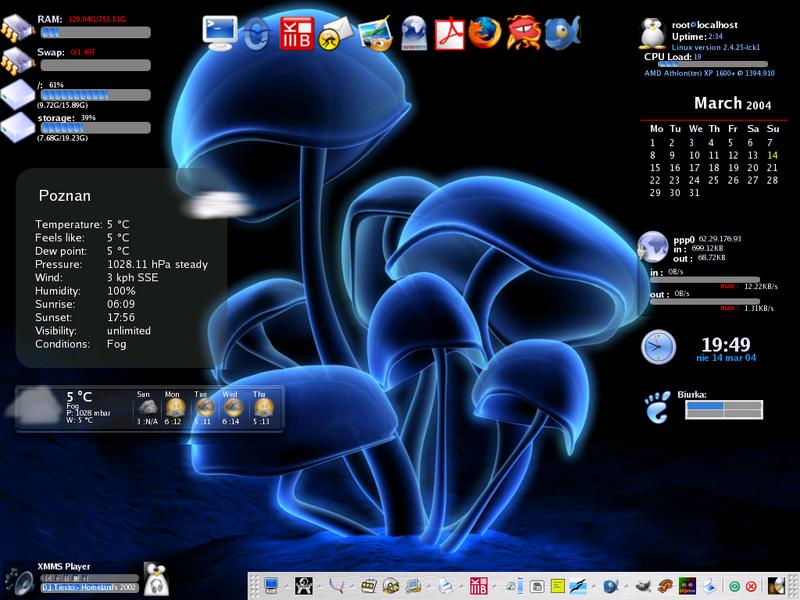
\includegraphics[height=3.5cm]{img/C03_estructura/gui_xfce}}
	\subfigure[LXDE]{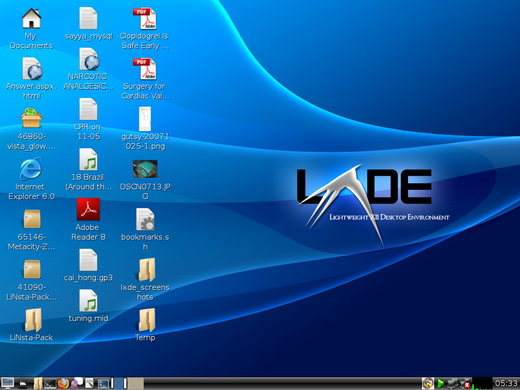
\includegraphics[height=3.5cm]{img/C03_estructura/gui_lxde}}
	\subfigure[Fluxbox]{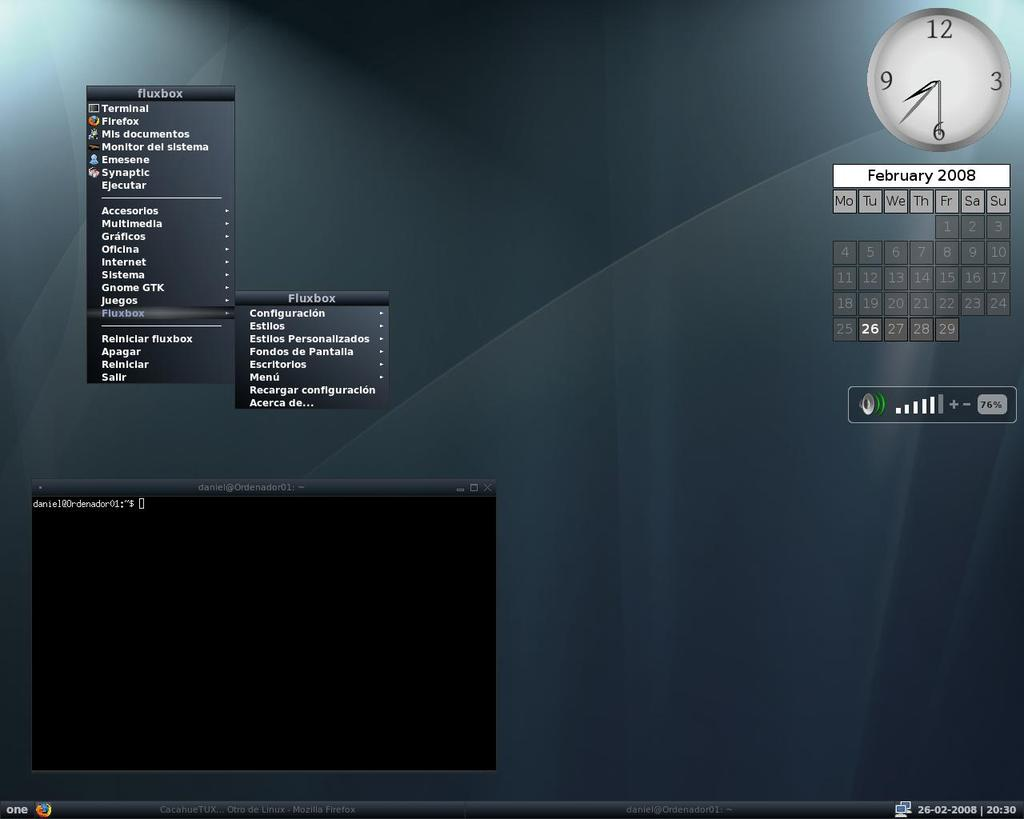
\includegraphics[height=3.5cm]{img/C03_estructura/gui_fluxbox}}
\end{center}
\caption{Diversos entornos gráficos}
\label{gui}
\end{figure}

\section{API y llamadas al sistema}
Las \textbf{llamadas al sistema} corresponden a una interfaz para utilizar los
servicios del sistema operativo, algunos ejemplos de estos son:

\begin{itemize}

	\item Errores de procesos (hardware o software).

	\item Lectura, creación o borrado de archivos.

	\item Imprimir texto por pantalla.

	\item Acceso a dispositivos de E/S.

\end{itemize}

Una \textbf{API} o \textit{Aplication Program Interface} corresponde al conjunto
de intrucciones y procedimientos que se ofrecen como biblioteca. En el caso del
sistema operativo, es la biblioteca que entrega las funciones que permiten hacer
uso de las llamadas al sistema.

La API es dependiente del sistema operativo, y algunos ejemplos de estas son la
API POSIX\footnote{Portable Operating System Interface, utilizada en sistemas
\textit{like Unix}}, la API Win32 y la API de Java.

La principal ventaja de utilizar una API para el desarrollo de aplicaciones
tienen que ver con la abstracción que el programador realiza del sistema, donde
no necesita conocer a fondo el mismo y puede generar una menor cantidad de
código e instrucciones más simples. Lo anterior implica una mayor facilidad al
momento de portar el código desde un sistema operativo (o máquina) a otro(a).

\subsection{Tipos de llamadas al sistema}
Las llamadas a sistemas se pueden dividir en cinco grupos principales, los
cuales corresponden a control de procesos, manipulación de archivos,
manipulación de dispositivos, mantenimiento de información y comunicaciones.
Estas serán discutidas a continuación.

\subsubsection{Control de procesos}
Estas llamadas a sistema se encargan de diferentes tareas que tienen relación
con los estados y vida de un proceso.

Por ejemplo se debe manejar el \textbf{término} donde en caso de errores se
podrá producir un volcado de memoria y el programador deberá proceder a depurar
el programa, por ejemplo utilizando una herramienta como gdb. En el caso de
término el sistema operativo deberá pasar a la siguiente tarea a realizar,
generalmente planificando un nuevo proceso. En caso del retorno de salida,
existen distintos niveles de error, donde el estándar es que 0 corresponde a un
retorno normal y cualquier valor positivo a un error, donde entre más alto el
número más grave debiese ser el error.

También se deben manejar temas relacionados con la \textbf{carga y ejecución}
del proceso, donde puede ser necesario cargar y/o ejecutar otro programa, por
ejemplo cuando un proceso $A$ llama a un proceso $B$. Una vez termina la
ejecución del proceso $B$ el control debería volver al proceso $A$. Esto último
se observa claramente al ejecutar un comando en un intérprete, ya que al
ejecutar, por ejemplo, el comando $ls$ cuando este termine el control volverá al
intérprete.

Otra llamada al sistema tiene relación con los \textbf{atributos de procesos},
donde el sistema operativo deberá obtener y fijar los mismos, como prioridad o
tiempo máximo de ejecución del proceso. \textbf{Tiempos de espera} los cuales
son determinados por un tiempo $X$ de espera o bien por la espera de algún
suceso que se requiera. O llamadas al sistema para la asignación de
\textbf{memoria principal}.

La llamada al sistema \textbf{\textit{kill}} permite enviar señales a los
procesos. Estas señales envían una instrucción al proceso con diferentes
objetivos, por ejemplo para matar el proceso (KILL), terminar el proceso (TERM),
suspender el proceso (STOP) o ejecutar una alarma (ALRM). Para enviar una señal
en sistemas \textit{like Unix} se utiliza el comando \textit{kill}.

Algunos ejemplos de llamadas al sistema relacionadas son \texttt{fork} (crea un
proceso hijo), \texttt{exec} (carga programa en memoria y ejecuta),
\texttt{wait} (espera hasta la finalización del proceso hijo) y \texttt{exit}
(termina la ejecución del proceso).

\subsubsection{Manipulación de archivos}
Las llamadas a sistema relacionadas con la manipulación de archivos tienen
principalmente las funciones de realizar \textbf{operaciones básicas sobre
archivos} y \textbf{determinar atributos o cambiarlos}, como el nombre el tipo
del archivo, los permisos que tiene un usuario, etc.

Algunos ejemplos de llamadas al sistema relacionadas son \texttt{create},
\texttt{delete}, \texttt{open}, \texttt{read}, \texttt{write},
\texttt{reposition} y \texttt{close}.

\subsubsection{Manipulación de dispositivos}
Permiten controlar el acceso a los dispositivos, el cual debe ser controlado, si
un proceso requiere un recurso y este está ocupado el proceso deberá esperar por
el recurso.

Los dispositivos que se deberán manipular pueden ser tanto físicos, como el
disco duro, y virtuales, como archivos. En sistemas \textbf{like Unix} los
dispositivos pueden ser encontrados en el directorio \texttt{/dev}.

Algunos ejemplos de llamadas al sistema relacionadas son \texttt{request},
\texttt{release}, \texttt{open}, \texttt{close}, \texttt{read}, \texttt{write} y
\texttt{reposition}.

\subsubsection{Mantenimiento de información}
El propósito de estas llamadas al sistema es transferir datos entre el programa
de usuario y el sistema operativo. Ejemplos de estos tipos de datos son tiempo,
usuarios, versión S.O., memoria libre (o disco duro), etc. Información general
del funcionamiento del sistema operativo puede ser encontrada, en sistemas
\textit{like Unix}, en el directorio \texttt{/proc}.

Algunos ejemplos de llamadas al sistema relacionadas son \texttt{time},
\texttt{date} y \texttt{sysinfo} (usada por comando \texttt{uname}).

\subsubsection{Comunicaciones}
En este tipo de llamadas al sistema se incluyen aquellas que permiten realizar
la comunicación entre procesos, por ejemplo mediante el \textbf{modelo por paso
de mensajes}, usando sockets o el \textbf{modelo de memoria compartida}, donde
se debe eliminar la restricción del sistema operativo que protege datos en
memoria en el caso de proceso pesados.

Algunos ejemplos de llamadas al sistema relacionadas son \texttt{get\_hostid},
\texttt{get\_processid}, \texttt{open}, \texttt{close},
\texttt{accept\_connection}, \texttt{wait\_for\_connection},
\texttt{read\_message}, \texttt{write\_message}, \texttt{shared\_memory\_create}
y \texttt{shared\_memory\_attach}.

\section{Diseño}
Durante el diseño del sistema operativo se deberá considerar que los
dispositivos sean mapeados en la memoria del computador como si fuesen
posiciones en ella, si se lee en dicha dirección de memoria, en el fondo, se
accede al dispositivo en si, análogamente si se escribe en esa dirección de
memoria se hará escritura en el disco. Esto es básicamente los que sucede con
los ficheros que se encuentran en \texttt{/dev} que representan dispositivos
físicos de la máquina.

% ejemplo disco duro e interrupciones
Sigamos con el ejemplo del disco, una vez terminada la ejecución de la rutina
llamada para realizar la lectura no significa que se haya realmente terminado de
leer desde el disco. En realidad la rutina que se ejecuta es el comando que se
introduce para que se inicie la verdadera lectura y el disco tiene su propio
microcontrolador que se encarga de realizar la operación. La CPU consultará
entonces reiteradamente para verificar si se completo o no la lectura en un
ciclo conocido como \textit{busy-waiting}, esto es lo que sucedía originalmente
en los primeros sistemas operativos como ya fue discutido anteriormente en el
capítulo \ref{historia}. El problema de este enfoque es que se pierde tiempo
mientras se realiza la operación de lectura, alrededor de 10 [ms], donde no se
hace otro trabajo útil.

Mucho mejor podría ser ejecutar otros procesos, mientras se espera que se lea el
disco, y se obtengan los datos que requiere el proceso para continuar. En este
caso el proceso quedará bloqueado y deberá esperar a que el sistema operativo le
notifique que los datos solicitados ya se encuentran listos para su uso.

El uso de interrupciones permite al disco avisar a la CPU que la operación en
disco terminó, se suspende al proceso que está actualmente en la CPU y se
ejecuta una rutina para atender la interrupción. Esta rutina de atención informa
al proceso que lo solicitado del disco ya está disponible y se pasa el proceso a
un estado listo para esperar a ser planificado nuevamente.

Existe dentro del núcleo del sistema operativo un vector de interrupciones con
todas las posibles fuentes de las mismas, como de disco o las del
\textbf{cronómetro regresivo}.

Un proceso que se esta ejecutando podría acaparar la CPU, entonces el sistema
operativo utiliza la interrupción del cronómetro regresivo para interrumpir al
proceso que se está ejecutando, por ejemplo después de 10 o 100 [ms], y asignar
la CPU a otro proceso, con este mecanismo se implementan las \textbf{tajadas de
tiempo}. Si estas son suficientemente pequeñas el usuario tendrá la sensación
que todo avanza al mismo tiempo, o sea, ``ejecución en paralelo''.

Otros ejemplos de interrupciones son aquellas que ocurren al hacer divisiones
por 0 o la ejecución de instrucciones ilegales (código de operación indefinida,
operación que no existe en el procesador o operación privilegiada).

No confundir interrupciones con señales, estas son ``interrupciones virtuales''
y su ámbito es en los procesos. Cada proceso maneja su propio cronómetro
regresivo virtual. El núcleo tiene una agenda con todas las señales que debe
generar y revisa cual es la próxima que debe ocurrir y entonces el cronómetro
regresivo coloca la alarma a dicha señal que se requiere para dicho proceso.
Mandar una señal a un proceso implica activar el proceso para que este pueda
atender la señal.
% fin ejemplo interrupciones

Otro aspecto a considerar en el diseño del sistema operativo son los canales que
se utilizan para acelerar la entrada y salida de datos, que pueden ayudar a
transferir muy rápido los datos. Lo anterior se logra utilizando un mecanismo
del mismo hardware que permite hacer una transferencia directa entre
dispositivos y memoria. Una vez terminada la transferencia se genera una
interrupción que indica que los datos ya están en la memoria. Con lo anterior el
núcleo evita tener que mover los datos desde el dispositivo a la memoria, esta
tarea la realiza el canal. Estos canales son conocidos como DMA o \textit{Direct
Memory Access}, donde el dispositivo, a través de este mecanismo, accede
directamente a la memoria.

\subsection{Objetivos}
Se deben definir objetivos y especificaciones, por ejemplo el hardware que se
requerirá y el tipo de sistema operativo que se desea implementar. Estos se
dividirán en objetivos del usuario y objetivos del sistema.

El \textbf{usuario} esta preocupado por que el sistema operativo sea cómodo de
utilizar, fácil de aprender y usar, fiable, seguro y rápido.

El \textbf{sistema} esta preocupado por que el sistema operativo sea flexible,
fiable, libre de errores, eficiente, fácil de diseñar, implementar y mantener.

Los objetivos tanto de usuario como de sistema a veces pueden no ser
compatibles, por ejemplo, para ser muy eficiente, quizás se deba sacrificar
usabilidad. Por lo anterior es que se deberá encontrar un equilibrio entre los
objetivos de ambos lados.

\subsection{Políticas y mecanismos}
Se deben definir \textbf{políticas} que indicarán \textbf{¿qué hacer?} y
\textbf{mecanismos} que indicarán \textbf{¿cómo hacerlo?}. Es recomendable que
políticas y mecanismos se encuentren separados, esto permitirá tener una mayor
flexibilidad ya que si se desea modificar una se puede minimizar el impacto en
la otra.

Las políticas determinarán todas las decisiones que el sistema operativo debe
tomar. Por ejemplo si se debe o no asignar un recurso, deberá existir una
política que indique cuando se aceptará la asignación y cuando se rechazará.
Asociado a esta política debe ir un mecanismo que indique como hacer la
asignación o como indicar el rechazo.

\subsection{Requerimientos para protección de procesos}
La \textbf{protección de procesos} significa que un proceso no debería
interferir con otros procesos, un proceso que esta corriendo no debería poder
acceder a los datos que otro esta manipulando. Ejemplos de estos sistemas
operativos son Unix y Windows NT, y los derivados de ambos.

\subsubsection{Modo dual}
En esta forma de operación se deben implementar dos modos básicos en que el
sistema operativo debe funcionar. El primero corresponde al \textbf{\textit{user
mode}}, o modo usuario o no privilegiado, en donde se ejecutan todos los
procesos, incluyendo aquellos que son ejecutados por el usuario root. Este modo
tiene ciertas restriccioens que impiden que un usuario pueda ejecutar cualquier
instrucción o código en la máquina, por ejemplo la instrucción que permite
deshabilitar las interrupciones. Si este modo no existiese un proceso cualquiera
podría desactivar, por ejemplo, el cronómetro regresivo, y evitar que otros
ocupen la CPU. En este modo, dicha instrucción es privilegiada, por lo cual al
ejecutarse ocurriría una interrupción de software (interrupción de comando
ilegal).

Es importante notar que a pesar de estar en modo usuario uno si podría
desactivar las señales en procesos (no ignorar, desactivar), excepto la señal
KILL. Si el proceso recibe una señal, la interrupción asociada ocurrirá pero el
sistema operativo no la entregará al proceso hasta que estén habilitadas
nuevamente. Importante mencionar que solo se desactivan señales de ese proceso,
ya que al ser modo usuario un proceso no puede interferir con otro.

El otro modo corresponde al \textbf{\textit{kernel mode}}, modo sistema, modo
supervisor o modo privilegiado. En este modo todo es permitido, por ejemplo aquí
si se podrían desactivar las interrupciones. El núcleo es el único que corre
sobre modo sistema, incluyendo sus módulos. Importante mencionar que dentro del
núcleo no hay \textit{segmentation fault}, en caso de existir algún error podría
derivar en un \textit{kernel panic}, es por esta razón que solo el usuario root
puede cargar módulos al núcleo.

En la figura \ref{modo_dual} se ilustra cada una de las partes que están
involucradas en el modo usuario y el modo sistema en GNU/Linux. Las aplicaciones
de los usuarios y la API glibc corren sobre el modo usuario, mientras que las
llamadas a sistema, el núcleo y las instrucciones directas al hardware lo hacen
en modo sistema. Si un usuario requiere hacer uso de una llamada a sistema
deberá hacerlo a través de la API correspondiente, entonces el sistema operativo
concederá solo por la ejecución de esa parte del código acceso a modo sistema,
revocándoselo una vez la instrucción termine y siguiendo su ejecución en modo
usuario. Es importante destacar que un usuario normal no puede acceder
llamadas de sistema privilegiadas, se requiere ser usuario root para esto.

\begin{figure}[htbp]
\begin{center}
	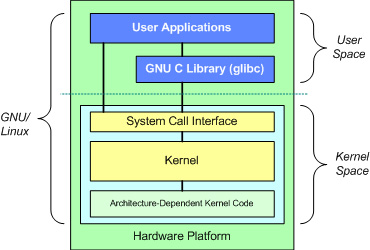
\includegraphics[scale=1.0]{img/C03_estructura/modo_dual}
	\caption{Componentes presentes en el modo usuario y el modo sistema}
	\label{modo_dual}
\end{center}
\end{figure}

\subsubsection{Unidad de gestión de memoria}

La \textbf{MMU} o \textit{Memory Management Unit} básicamente lo que hace es
traducir de direcciones virtuales a direcciones reales. Las direcciones
utilizadas por los procesos son virtuales, varios pueden usar la dirección 0x3A,
pero cuando se mapean a la memoria real se mapean a direcciones físicas
distintas, esto lo hace la MMU. Esto será cubierto en detalle en el capítulo
\ref{memoria_principal}.

Los primeros procesadores para computadores personales que aparecieron con MMU
fueron los x86, a mediados de los años 80s. Antes ya habían equipos con MMU,
pero eran los \textit{mainframes}\footnote{Computadoras grandes, potentes y
costosas utilizados en grandes instituciones}, ya que estos eran para
sistemas multiusuarios. Como ejemplo de sistemas operativos que la requieren
esta Unix que al ser multiusuario necesita MMU, Linux es derivado de Unix por lo
que también la requiere y Android al ser derivado de Linux igualmente la
necesita.

\section{Estructura del sistema operativo}
Se deberá elegir un método para estructurar las funcionalidades que se
proveerán. Actualmente los sistemas operativos se encuentran divididos por
jerarquías con funciones bien definidas. Se mencionarán algunas formas de
estructurar el sistema a continuación.

\subsection{Estructura simple}
La estructura simple esta orientada a sistemas operativos pequeños, simples y a
su vez limitados.

Por ejemplo, MS-DOS entregaba máximas funcionalidades en un tamaño reducido, no
poseía una división cuidadosa de sus módulos. Adicionalmente dicho sistema
operativo entregaba acceso directo a rutinas que podían utilizar el hardware,
por lo cual no se considera un sistema operativo con protección de sus procesos.

En el caso del Unix original, el kernel a través de las llamadas al sistema
provee las funcionalidades necesarias para acceder a los recursos.

\subsection{Estructura en niveles}
En este tipo de estructuras se utiliza un método de diseño arriba-abajo, el
sistema resultante corresponderá a un sistema por niveles donde la estructura
jerárquica se determinará de acuerdo a la complejidad de las funciones de cada
nivel.

Las ventajas de utilizar esta estructura radica en la independencia que se
conseguirá entre los niveles, ya que cada uno se encargará de una tarea
específica que le entregará servicios a otro nivel. Se debe preocupar mantener
las mismas funcionalidades que se entregan a otras capas, no importando como se
cambie esto internamente. Esto proporciona facilidad en la construcción,
mantención y depuración del sistema operativo.

Se debe tener especial cuidado en la definición apropiada de los diferentes
niveles, donde esto debe hacerse de forma correcta para lograr la independencia
anteriormente mencionada. Además se debe considerar que ciertas capas podrán
depender de otras para operar. Una desventaja es que al introducir niveles la
operación total podría resultar un poco más lenta, ya que se deben utilizar
interfaces entre las diferentes capas del sistema.

A continuación se muestra un ejemplo de los posibles niveles de jerarquía para
un sistema operativo. Notar los niveles del 1 al 4 no corresponden directamente
a funciones del sistema operativo, estas son realizadas por hardware. También
observar que las capas superiores requerirán servicios de capas inferiores como
es el caso del nivel de directorios que requiere servicios de la capa sistema de
archivos y esta a su vez de la capa de almacenamiento secundario.

\begin{enumerate}

	\item Circuitos electrónicos: registros, puertas, buses.

	\item Instrucciones: evaluación de la pila, microprogramas, vectores de
	datos.

	\item Procedimientos: pila de llamadas, visualización.

	\item Interrupciones: manejo de interrupciones del hardware.

	\item Procesos primitivos: semáforos, colas de procesos.

	\item Almacenamiento secundario: bloques de datos.

	\item Memoria virtual: paginación.

	\item Comunicaciones: tuberías.

	\item Sistema de archivos: almacenamiento en disco duro u otro medio.

	\item Dispositivos: impresoras, pantallas, teclados.

	\item Directorios: árbol de directorios.

	\item Procesos de usuario: programas en ejecución.

	\item Shell: intérprete de comandos.

\end{enumerate}

\subsection{\textit{Microkernels}}
Un sistema operativo que está organizado como micro núcleo entrega solo las
tareas básicas, como: planificación de procesos, gestor de memoria y
comunicaciones. Otras tareas son realizadas por programas del sistema operativo
y el núcleo es utilizado como un intermediario para la comunicación entre el
usuario y los programas del sistema operativo que ofrecen los servicios.

Los programas nuevos para el sistema operativo son añadidos al espacio del
usuario, se ejecutan en modo usuario y no como modo sistema. El núcleo entonces
se encarga de realizar las llamadas al sistema a través de mensajes hacia los
servicios correspondientes que entregan las funcionalidades solicitadas.

Su ventaja es que al incorporar las mínimas funcionalidades, son más estable.
Sin embargo la principal desventaja en este tipo de núcleos es que son
ineficientes al tener que realizar muchos cambios de contexto para ir a los
servicios prestados.

Minix es un ejemplo de este tipo de sistema operativo.

\subsection{Módulos}
En este caso el sistema operativo está compuesto por módulos, donde lo
fundamental se encuentra en el núcleo en si, pero otras funcionalidades son
entregadas como módulos del núcleo. Ambos, tanto el núcleo como los módulos
corren en modo sistema.

Esto permite que componentes sean cargados dinámicamente al núcleo, evitando
tener que disponer del soporte para todos los dispositivos o funcionalidades
permanentemente cargados en memoria principal. En Linux esto se puede realizar
mediante el uso de las instrucciones \texttt{lsmod}, \texttt{modprobe} y
\texttt{rmmod}.

Algunos ejemplos de módulos que pueden existir son controladores de disco,
controladores de tarjetas de red o el soporte para IPv6. Es importante mencionar
que el soporte necesario para que la máquina pueda ser arrancada, en estricto
rigor para que el disco duro que contiene el sistema raíz del sistema operativo
sea abierto, no puede ir como módulo del núcleo. Lo anterior ya que los módulos
se cargan cuando el sistema esta iniciando, una vez que ya se montó el sistema
de archivos.

Ejemplos de estos sistemas operativos son Unix modernos, Solaris, Linux y Mac
OSX.

Se hablará más adelante de módulos en Linux en el capítulo \ref{linux_modulos}.

\section{Implementación}
Una vez se decide la estructura del sistema operativo y están definidas las
políticas del mismo se debe realizar la implementación. Originalmente esto se
realizaba programando el hardware de la máquina, posteriormente se utilizaba un
lenguaje de bajo nivel o lenguaje de máquina (\textit{assembler}) y actualmente
se utilizan lenguajes de alto nivel (como C o C++).

La principal ventaja de utilizar lenguajes de alto nivel radica en que es fácil
de programar, el código que se escribe es compacto, fácil de entender y depurar.
Adicionalmente las mejoras introducidas en los compiladores significarán mejoras
en el código generado, por lo tanto mejoras en el sistema operativo que se está
compilando. Finalmente colabora con la portabilidad de un sistema operativo de
un hardware a otro, recordar que será la API de cada lenguaje la que se
encargará de traducir las instrucciones a la arquitectura seleccionada.

Desde el punto de vista de la optimización del sistema operativo es recomendable
atacar a las estructuras de datos y algoritmos utilizados en tareas críticas,
tales como el planificador de la CPU y el gestor de memoria. Una vez
identificados los problemas se deben optimizar, por ejemplo reemplazando el
código de alto nivel por código de máquina.

\section{Ejercicios y preguntas}
\begin{enumerate}

	\item Mencione y explique 5 servicios que se deben considerar al momento
	de diseñar el sistema operativo.

	\item ¿Cuál es la diferencia entre CLI y GUI?.

	\item Mencione tres ventajas de utilizar una API.

	\item ¿Qué es una llamada al sistema?, de dos ejemplos (que no sea
	kill).

	\item La llamada sistema kill permite enviar señales a procesos, indique
	la diferencia entre la señal KILL y TERM.

	\item ¿Por qué \textit{busy-waiting} es ineficiente?.

	\item ¿Quién atiende las interrupciones?.

	\item ¿Para que es utilizado el cronómetro regresivo?.

	\item Explique la diferencia entre interrupciones y señales.

	\item Explique el concepto de modo dual, o sea, explique los modos
	usuario y sistema. Adicionalmente de ejemplos de cuando se utiliza cada
	uno de ellos.

	\item ¿Cuándo ocurre un cambio de modo usuario a modo sistema?.

	\item ¿Una aplicación puede ejecutar directamente una llamada al sistema
	sin utilizar una API?

	\item Explique la estructura de núcleo monolítico.

	\item Explique la estructura de \textit{microkernels}.

	\item Linux ¿a que tipo de estructura de sistema operativo corresponde?.

	\item ¿Cuál es la ventaja de utilizar un sistema con estructura
	modular?.

\end{enumerate}

\section{Referencias}
\begin{itemize}

	\item Sistemas Operativos, Segunda Edición, Andrew Tanenbaum, Capítulo
	1.3, 1.4 y 1.5.

	\item Sistemas Operativos, Quinta Edición, Abraham Silberschatz y Peter
	Baer Galvin, Capítulo 3.

\end{itemize}
